\documentclass[times, twoside, watermark]{zHenriquesLab-StyleBioRxiv}

% Note: Write each sentence on its own line (makes diffs easier to read).

% Please give the surname of the lead author for the running footer
\leadauthor{Khurana}

\begin{document}

%\title{pykarambola: a Python package for Minkowski tensor analysis of 3D triangulated surfaces}
\title{pykarambola: Minkowski tensor morphometry of 3D structures}
\shorttitle{pykarambola}

% Use letters for affiliations, numbers to show equal authorship (if applicable) and to indicate the corresponding author
\author[1]{Yajushi Khurana}
\author[1,\Letter]{Keisuke Ishihara}

\affil[1]{Department of Computational and Systems Biology, School of Medicine, University of Pittsburgh, Pittsburgh, PA, USA}
\maketitle

%TC:break Abstract
\begin{abstract}
% TODO (issue #22): Write abstract
\end{abstract}
%TC:break main

\begin{keywords}
Minkowski tensors | morphometry | 3D image analysis | Python | bioimage analysis
\end{keywords}

\begin{corrauthor}
ishihara\at pitt.edu
\end{corrauthor}


%% -------------------------------------------------------
\section*{Introduction}
%% -------------------------------------------------------

Three-dimensional morphometric analysis of biological structures requires shape descriptors that capture size, surface geometry, topology, elongation, and orientation in a mathematically principled way.
Minkowski functionals provide one such foundation: restricted to convex bodies in $\mathbb{R}^3$, Hadwiger's theorem states that every continuous, additive, and motion-invariant scalar functional is expressible as a linear combination of exactly four measures~\cite{SchroderTurk2013, HugSchneider2017}.
In three dimensions these are volume $V$, surface area $A$, integrated mean curvature $H$ (the surface integral of the mean of the two principal curvatures, quantifying average surface bending), and Euler characteristic $\chi$ (a topological invariant that counts connected components minus handles plus enclosed voids).
Together they provide a compact and complete description of size, surface extent, bending, and topology — yet being scalars they carry no directional information: a sphere, a cigar-shaped ellipsoid, and a flat disc can share identical $V$, $A$, $H$, and $\chi$ while differing profoundly in elongation and orientation.

Minkowski tensors are independent tensor-valued shape measures that extend this framework by accumulating directional contributions from the object's surface geometry~\cite{SchroderTurk2013, Beisbart2002, Schaller2020papaya2}.
The Cartesian Minkowski tensors $W_\nu^{r,s}$ encode orientation explicitly; for example, for the rank-2 surface tensor $W_1^{0,2}$ — which accumulates outer products of surface normals weighted by area — the ratio of smallest to largest eigenvalue defines the anisotropy index $\beta_0^{2,0}$: it equals one for a perfect sphere and decreases toward zero for increasingly elongated or oblate shapes.
A further layer of description comes from decomposing the Cartesian Minkowski tensors into irreducible representations under rotation, which gives rise to the Minkowski structure metrics $q_\ell$ and $w_\ell$: rotationally invariant quantities that characterise $\ell$-fold orientational order and have been applied extensively to detect crystal-like and liquid-crystalline local symmetry in colloidal and granular systems~\cite{SchroderTurk2013}.
Originally developed in structural physics, this hierarchy of shape descriptors — from scalar functionals through Cartesian tensors to structure metrics — is increasingly relevant in biological image analysis, where segmented structures such as nuclei and organelles often carry biologically meaningful elongation and orientation that scalar morphometrics cannot detect.
Realising this potential requires tools that integrate seamlessly into the workflows biologists already use.

% TODO (issue #25): Python ecosystem and bioimage analysis community
Modern bioimage analysis relies on open source tools largely written in Python.
A typical morphometry pipeline proceeds from microscopy acquisition through volumetric segmentation to quantitative shape measurement, with tools such as scikit-image~\cite{vanderwalt2014scikit} for image processing and surface extraction, napari~\cite{Sofroniew2026napari} for interactive 3D visualisation, and pandas~\cite{McKinney2010pandas} for tabular data handling.
Most morphometry tools in this ecosystem report simple scalar descriptors (volume, surface area, sphericity) that do not capture the directional properties of shape.
Approaches based on spherical harmonics~\cite{ruan2019evaluation, viana2023integrated} capture richer structural information but are restricted to genus-zero surfaces and do not generalise to objects with complex 3D topology.
Minkowski tensors capture directional information explicitly: their eigensystems directly quantify elongation and orientation, which are biologically relevant for polarised cells, elongated organelles, and anisotropic tissue architecture.
While computing Minkowski tensors on 3D triangulated surfaces is possible in C++ (karambola~\cite{Schaller2020karambola}), but it is not directly accessible within Python workflows.
Here we present our tool pykarambola, a Python package that integrates Minkowski tensor analysis directly into the Python bioimage ecosystem: in a single call, segmented objects are converted into triangulated surfaces and processed into a dict of NumPy arrays with the objects' corresponding Minkowski tensors, which makes its output immediately compatible with downstream analysis and mesh visualisation tools~\cite{Sofroniew2026napari, Sullivan2019pyvista, Musy2026vedo}.

% TODO (issue #24): karambola C++ and motivation for a Python port
The C++ karambola package~\cite{Schaller2020karambola} is the reference implementation for computing Minkowski tensors on 3D triangulated surfaces, and has been widely used in structural analysis of soft matter and disordered systems~\cite{SchroderTurk2013}.
It accepts meshes in two formats: the karambola-native \texttt{.poly} format and the Object File Format (\texttt{.off}), and writes results to plain-text files.
Despite its numerical capabilities, karambola is not distributed through a package manager, requires a C++ build toolchain, and provides no NumPy-compatible interface.
Since modern bioimage analysis pipelines operate predominantly in Python — with segmentation tools such as cellpose~\cite{Stringer2021cellpose} and scikit-image~\cite{vanderwalt2014scikit} producing in-memory NumPy arrays or integer label images — integrating karambola into such a workflow requires serialising data to disk in a supported mesh format, invoking the binary as a subprocess, and parsing the plain-text result files back into Python, adding fragile intermediates that are difficult to maintain.
pykarambola removes these barriers: it is installable with \texttt{pip install pykarambola}, extends input support to Wavefront OBJ (\texttt{.obj}) and binary glTF (\texttt{.glb}) in addition to \texttt{.poly} and \texttt{.off}, accepts vertex and face arrays directly as NumPy arrays, and returns results as plain Python dicts.



%% -------------------------------------------------------
\section*{Methods}
%% -------------------------------------------------------

\subsection*{Architecture of pykarambola}
pykarambola is a complete Python reimplementation of the C++ karambola package~\cite{Schaller2020karambola}.
The port reproduces the logical structure of the C++ source: a \texttt{Triangulation} class holds the surface mesh and precomputed per-triangle and per-edge geometry, a set of \texttt{calculate\_w*} functions implements the Minkowski tensor formulae, and a command-line interface reproduces the behavior of the original binary.
The C++ implementation depended on the GNU Scientific Library (GSL) for eigenvalue decomposition; pykarambola replaces this with NumPy's \texttt{eigh} routine, removing the only non-Python build dependency from the core computation.

The package is structured around a pure-Python core that requires NumPy~\cite{harris2020numpy} and SciPy~\cite{virtanen2020scipy}.
SciPy is used for connected component detection on mesh graphs and for spherical harmonic basis functions in the spherical Minkowski summary quantities (\texttt{msm}).
An optional Cython extension accelerates the graph-traversal steps of mesh initialisation; the package falls back to pure-Python implementations when the extension is absent (described below).
The API for computing Minkowski tensors directly from segmented 3D label images (\texttt{minkowski\_tensors\_from\_label\_image}) requires scikit-image~\cite{vanderwalt2014scikit} for marching-cubes surface extraction; this dependency is not declared as mandatory and resolves automatically in environments where scikit-image is already present.

Pykarambola retains support for the two mesh formats accepted by C++ karambola: the karambola-native \texttt{.poly} format and the Object File Format (\texttt{.off}).
Three additional parsers for Wavefront OBJ (\texttt{.obj}), binary glTF (\texttt{.glb}), and STereoLithography (\texttt{.stl}) were added to broaden compatibility with mesh files produced by common 3D reconstruction and visualisation tools.

The Python port and software development were assisted by AI language models (see Acknowledgements for disclosure).
Numerical correctness of the port was validated by extensive benchmarking against the C++ karambola binary across a diverse set of test meshes, confirming agreement to floating-point precision for all Minkowski scalars, vectors, and tensors.

\subsection*{Acceleration strategy: NumPy vectorization and Cython}
The primary performance strategy in pykarambola is NumPy vectorization~\cite{harris2020numpy}.
Rather than iterating over individual triangles or edges in Python, all mesh data are stored as contiguous NumPy arrays and bulk array operations are applied across the entire mesh at once.
During \texttt{Triangulation} construction, triangle normals, face areas, triangle centroids, edge lengths, and dihedral angles are precomputed in a single vectorized pass using batched cross-products and array-wise norm computations on $(F \times 3)$ arrays, where $F$ is the number of triangles.
Each Minkowski tensor function then reduces these precomputed arrays to per-label scalar, vector, or matrix accumulators using \texttt{numpy.sum} and \texttt{numpy.einsum}, with no Python-level loop over faces.

Two initialisation steps resisted vectorization: building the edge-keyed triangle-adjacency table and constructing the compressed-sparse-row vertex-to-triangle lookup table.
Both require sequential insertion into a hash map indexed by vertex-pair keys, a graph-traversal pattern with data-dependent branching that cannot be expressed as bulk array operations.
These two routines are therefore provided as an optional Cython extension (\texttt{\_accel.pyx}) that uses typed memoryviews and eliminates interpreter overhead on the inner loops.
When the extension is not installed, equivalent pure-Python implementations are used as a fallback.

\subsection*{High-level Python API}
pykarambola exposes two high-level functions that accept NumPy arrays and return plain Python dicts.
The first, \texttt{minkowski\_tensors}, accepts an $(V \times 3)$ vertex array and an $(F \times 3)$ integer face array and returns a dict whose string keys (\texttt{w000}, \texttt{w020}, \texttt{w020\_eigvals}, \ldots) map to NumPy scalars, vectors, or matrices.
The \texttt{compute} argument accepts \texttt{'standard'} (14 base tensors plus eigensystems), \texttt{'all'} (adds higher-order terms \texttt{w103}, \texttt{w104}, the spherical Minkowski summary quantities \texttt{msm}, and three pykarambola-specific derived scalars per rank-2 tensor: \texttt{\_beta}, the anisotropy index defined as the ratio of the smallest to the largest eigenvalue magnitude; \texttt{\_trace}, the matrix trace; and \texttt{\_trace\_ratio}, the trace divided by the corresponding Minkowski scalar, e.g.\ $\texttt{w020\_trace\_ratio} = \mathrm{Tr}(W^{0,2,0})/w^{0,0,0}$, which is defined only for the $W^{r,2,0}$ family where a paired scalar exists), or an explicit list of names for selective computation.
The boolean \texttt{compute\_eigensystems} (default \texttt{True}) controls whether eigendecomposition is performed for rank-2 tensors; setting it to \texttt{False} omits the \texttt{*\_eigvals} and \texttt{*\_eigvecs} keys and avoids six \texttt{numpy.eigh} calls per label, which can reduce runtime for large batch jobs that do not require eigensystems.
When the \texttt{labels} argument is provided as a per-face integer array, or set to \texttt{'auto'} to detect connected components automatically via SciPy, the function returns a nested dict keyed by label.
The optional \texttt{return\_count=True} argument changes the return value to a \texttt{(results, n\_objects)} tuple where \texttt{n\_objects} is the number of connected components counted by vertex-adjacency graph traversal, useful for detecting multi-component objects within a single label.
The \texttt{center} argument controls the reference point for position-dependent tensors: \texttt{None} uses the array origin, \texttt{'reference\_centroid'} reproduces the C++ karambola \texttt{--reference\_centroid} flag, \texttt{'centroid\_mesh'} shifts each object to its volume-weighted center of mass before computing, and an explicit $(3,)$ array applies a fixed shift; the boolean \texttt{center\_per\_label} (default \texttt{True}) determines whether centroid shifts are computed independently per labeled object or from the whole mesh.
The second, \texttt{minkowski\_tensors\_from\_label\_image}, accepts a three-dimensional integer NumPy array in which each nonzero value identifies an object.
It extracts a triangulated isosurface for each label via \texttt{scikit-image} marching cubes and returns a dict keyed by integer label with the same structure as the mesh API; the \texttt{spacing} argument propagates physical voxel dimensions to all length, area, and volume quantities, and \texttt{autolabel=True} treats the array as a binary mask and delegates connected-component splitting to the mesh API.


%% -------------------------------------------------------
\section*{Results}
%% -------------------------------------------------------

\begin{figure*}
\centering
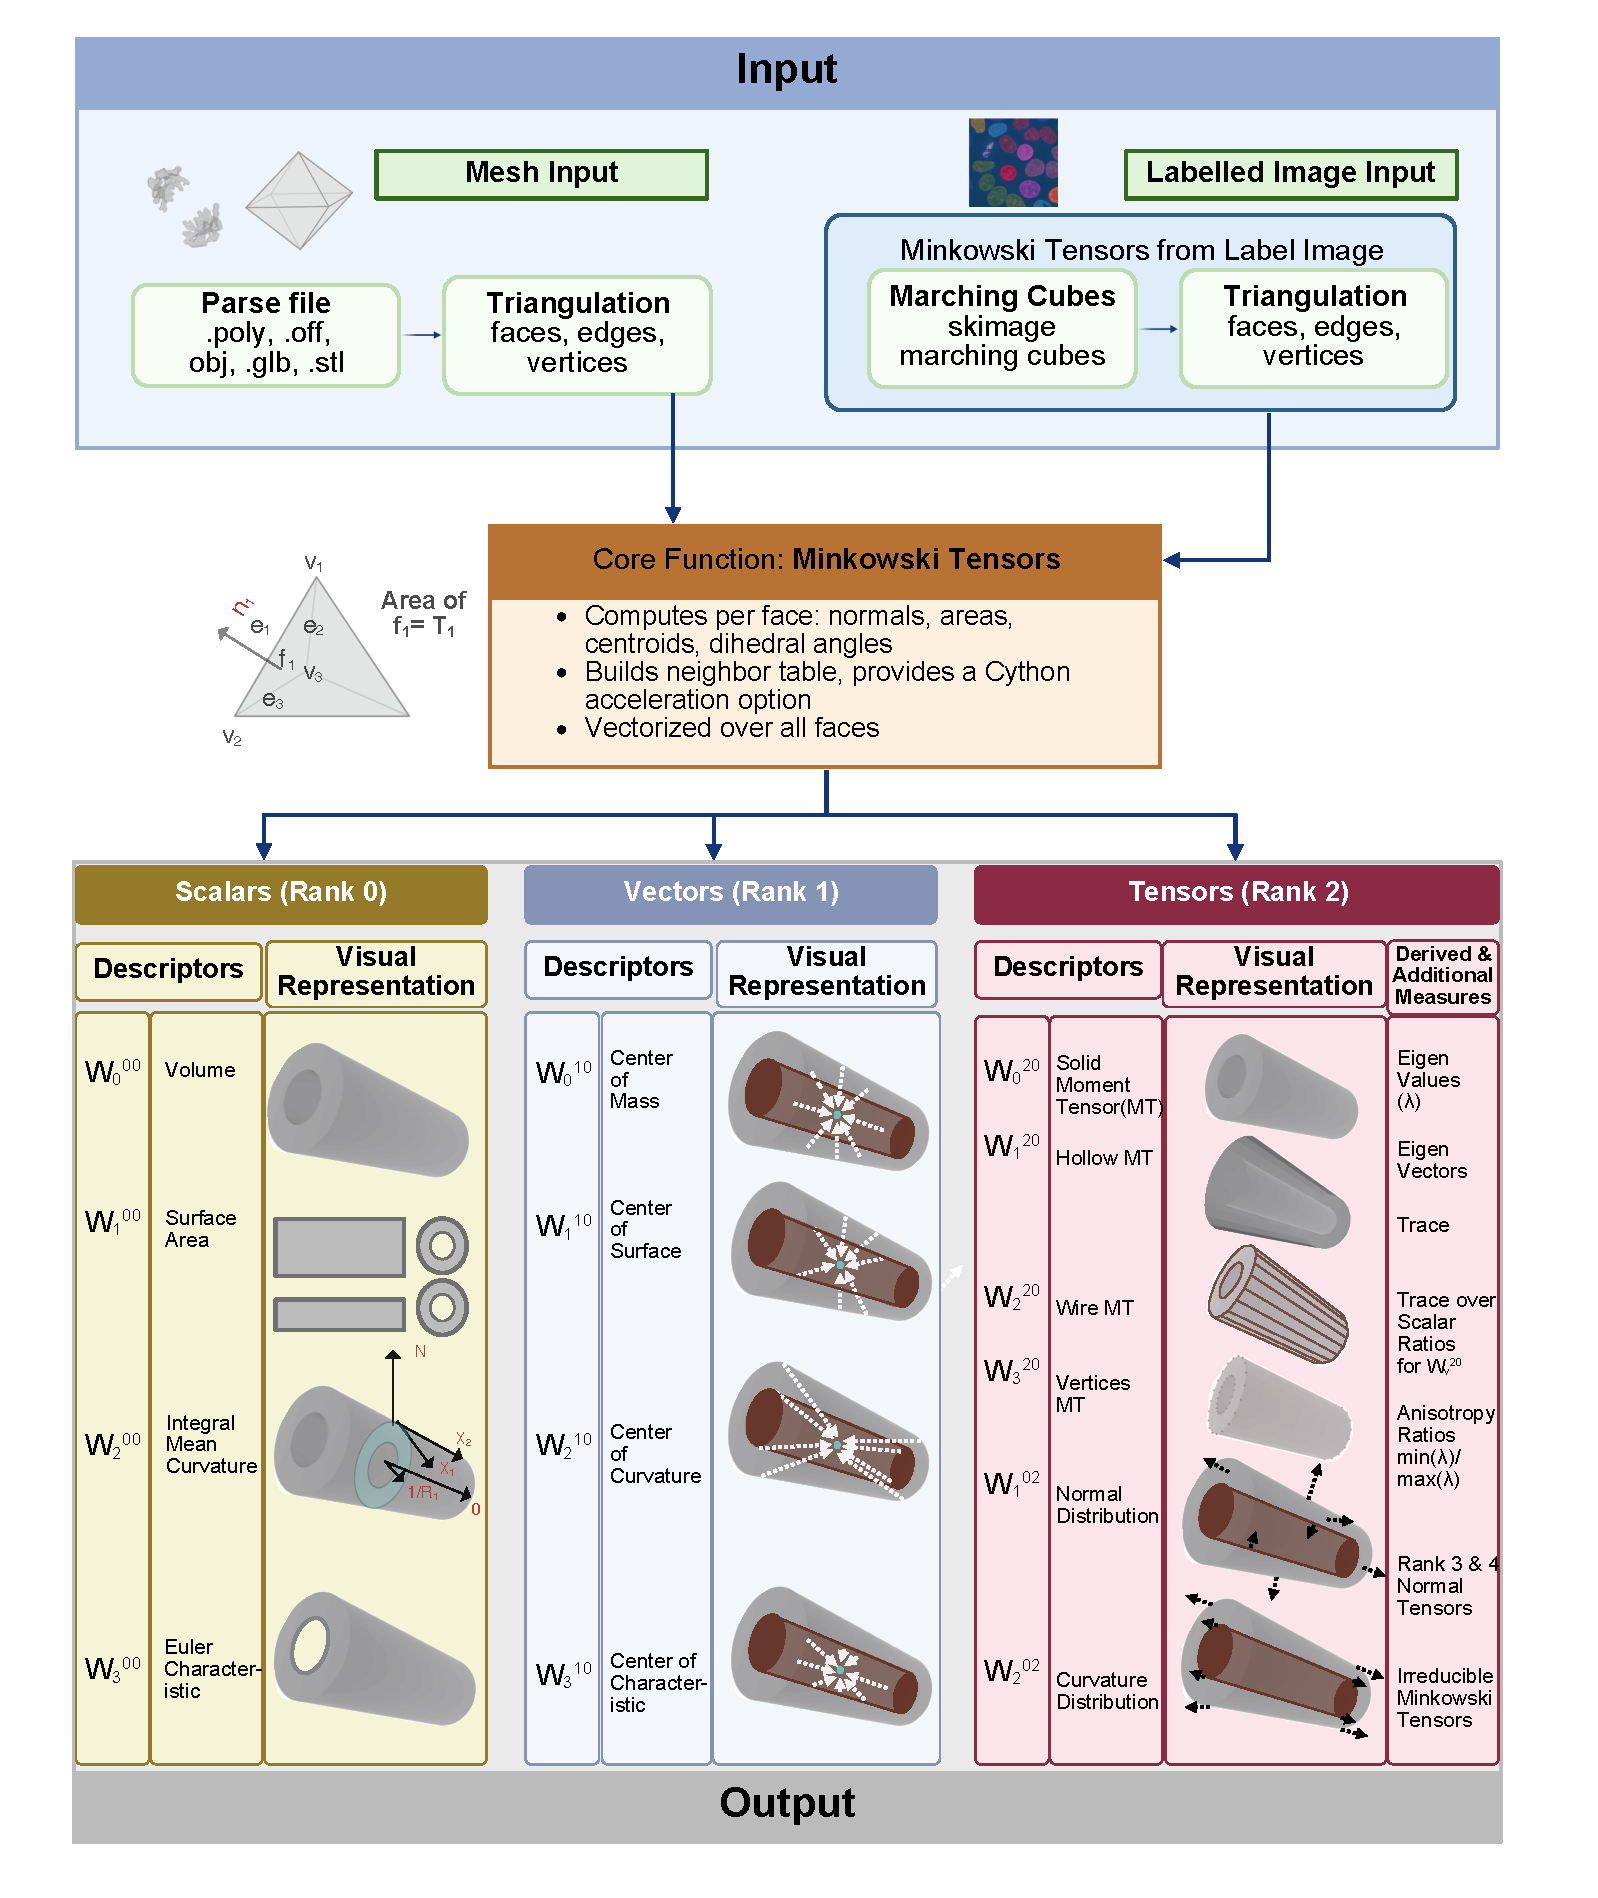
\includegraphics[width=0.95\textwidth]{../assets/pipeline_figure18.pdf}
\caption{%
  Computation pipeline of pykarambola.
  Two entry paths feed into a shared core:
  \texttt{minkowski\_tensors\_from\_label\_image} (left) accepts a 3D integer label image,
  pads the array, extracts an isosurface per label via marching cubes, and optionally
  centers each mesh;
  mesh files (\texttt{.poly}, \texttt{.off}, \texttt{.obj}, \texttt{.glb}) or direct
  \texttt{Triangulation} objects (right) bypass this step.
  The shared core constructs a \texttt{Triangulation} from vertex and face arrays,
  precomputes per-triangle and per-edge geometry in a single vectorised pass,
  and evaluates the Minkowski tensor functionals.
  Outputs are organised into three families:
  scalars ($w^{0,0,0}$, $w^{1,0,0}$, $w^{2,0,0}$, $w^{3,0,0}$),
  vectors ($w^{r,1,0}$),
  and rank-2 tensors ($w^{r,2,0}$ and $w^{r,0,2}$) with their eigensystems
  and anisotropy index~$\beta$.
}
\label{fig:pipeline}
\end{figure*}

\subsection*{Runtime benchmark}

We benchmarked pykarambola against the reference C++ karambola binary on two mesh sets.
First, synthetic icospheres at subdivision levels 5–10 (10{,}242 to 10{,}485{,}762 vertices) were used to characterise runtime scaling; both the pure-Python build and the Cython-accelerated build were timed independently (see Acceleration strategy, Methods).
Second, the AdrenalMNIST3D a standardized biomedical dataset~\cite{Yang2023MedMNIST} with 1{,}584 adrenal glands at two voxel resolutions (28$^3$ and 64$^3$) was used to measure performance on realistic biological meshes.
All measurements were performed on a single core of an Apple~M4 processor (macOS~15.7.3, Python~3.13, pykarambola~v0.5.0).

End-to-end (file parse plus compute), both \texttt{pykarambola} builds achieved 
runtimes within $1.0$--$1.3\times$ of C++ \texttt{karambola} across all mesh 
sizes tested (Figure~\ref{fig:runtime}). The Cython-accelerated build 
(\texttt{pykarambola[accel]}) was consistently faster than \texttt{karambola} 
($1.0$--$1.2\times$ speedup; Figure~\ref{fig:runtime}b, orange), while the 
pure-Python build showed comparable or slightly slower runtimes at larger mesh 
sizes ($0.8$--$1.0\times$; Figure~\ref{fig:runtime}b, blue). Within 
\texttt{pykarambola}, the Cython acceleration reduced compute time by 
$1.2$--$1.3\times$ relative to the pure-Python build, with the benefit most 
pronounced at larger mesh sizes.

On AdrenalMNIST3D, \texttt{pykarambola} processed all 1{,}584 meshes at 
$28^3$ resolution in 11~s versus 31~s for C++ \texttt{karambola} 
($2.8\times$ faster) and at $64^3$ resolution in 61.8~s versus 90~s 
($1.5\times$ faster). Note that the C++ \texttt{karambola} timing includes 
sequential file I/O (one result folder per mesh written to disk), whereas the 
\texttt{pykarambola} timing covers only in-memory computation; the file I/O 
overhead of the C++ binary accounts for most of the speedup observed on the 
adrenal dataset.

\begin{figure*}
\centering
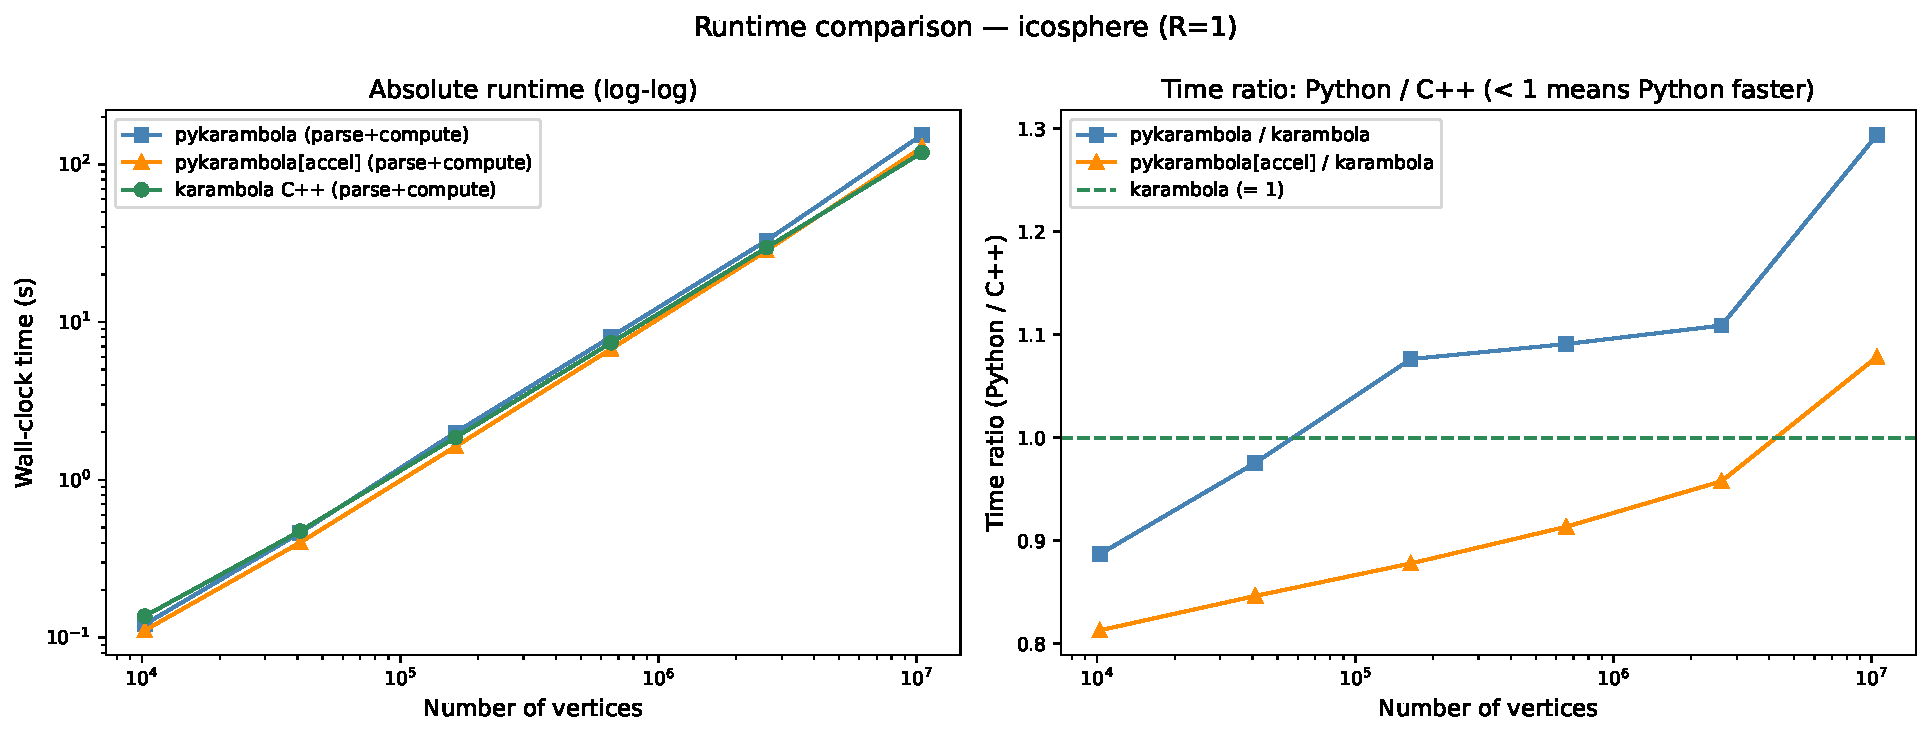
\includegraphics[width=\textwidth]{notebooks/results/timing_comparison_option_a.pdf}
\caption{Runtime benchmark on synthetic icospheres (subdivision levels 5--10; 10{,}242--10{,}485{,}762 vertices).
\textbf{Left}: absolute wall-clock time (log-log scale) for end-to-end execution (mesh parse + Minkowski tensor compute) for C++ karambola (green), pykarambola pure-Python (blue), and pykarambola Cython-accelerated (orange).
\textbf{Right}: speedup ratio (karambola time / pykarambola time); values above the dashed line ($= 1$) indicate pykarambola is faster.}
\label{fig:runtime}
\end{figure*}

\subsection*{Numerical accuracy}

We compared \texttt{pykarambola} output to C++ \texttt{karambola} on the full 
AdrenalMNIST3D dataset~\cite{Yang2023MedMNIST} (1{,}584 meshes at both $28^3$ 
and $64^3$ resolutions), evaluating all 121 scalar values output by 
\texttt{karambola}: 4 Minkowski scalars, 12 vector components, 36 rank-2 tensor 
upper-triangle elements, 18 rank-2 tensor eigenvalues, 27 components of the 
rank-3 tensor $W^{1,0,3}$ (\texttt{w103}), 6 eigenvalues of $W^{1,0,4}$ 
(\texttt{w104}), and 18 spherical Minkowski summary values (\texttt{msm\_ql}, 
\texttt{msm\_wl}).

Tensor eigenvectors are computed by \texttt{pykarambola} but are excluded from 
direct comparison: eigenvectors are defined only up to sign and, in the presence 
of degenerate eigenvalues, up to arbitrary rotation within the degenerate 
subspace; the eigenvalues fully characterise the spectral geometry of each tensor.

Across all 121 features, all 1{,}584 meshes, and both resolutions, 
\texttt{pykarambola} and \texttt{karambola} outputs fall on the identity line 
(Figure~\ref{fig:accuracy}). Residual discrepancies are consistent with 
floating-point summation order differences between the C++ and Python 
implementations and with the substitution of the GNU Scientific Library 
eigenvalue solver with NumPy's \texttt{eigh}. The maximum mean absolute 
difference across all features was $1.6 \times 10^{-4}$, observed for 
$W_2^{2,0}$ diagonal components at $64^3$ resolution; all remaining features 
agree to within $5 \times 10^{-9}$ on average.

The spherical Minkowski summary quantities (\texttt{msm\_ql} and 
\texttt{msm\_wl}, $l = 0, \ldots, 8$) show a distinct accuracy pattern 
(Figure~\ref{fig:accuracy}). For \texttt{msm\_ql} and even-$l$ 
\texttt{msm\_wl}, both implementations agree to floating-point precision. 
For odd-$l$ \texttt{msm\_wl} ($l = 1, 3, 5, 7$), the Wigner 3j parity 
selection rule requires $w_l = 0$ exactly. \texttt{pykarambola}'s Racah-formula 
implementation applies this rule analytically and returns exactly zero, whereas 
C++ \texttt{karambola} uses \texttt{gsl\_sf\_coupling\_3j}, which evaluates 
numerically without an explicit parity check, producing spurious residuals of 
order $10^{-8}$--$10^{-7}$ on the AdrenalMNIST3D meshes.

\begin{figure*}
\centering
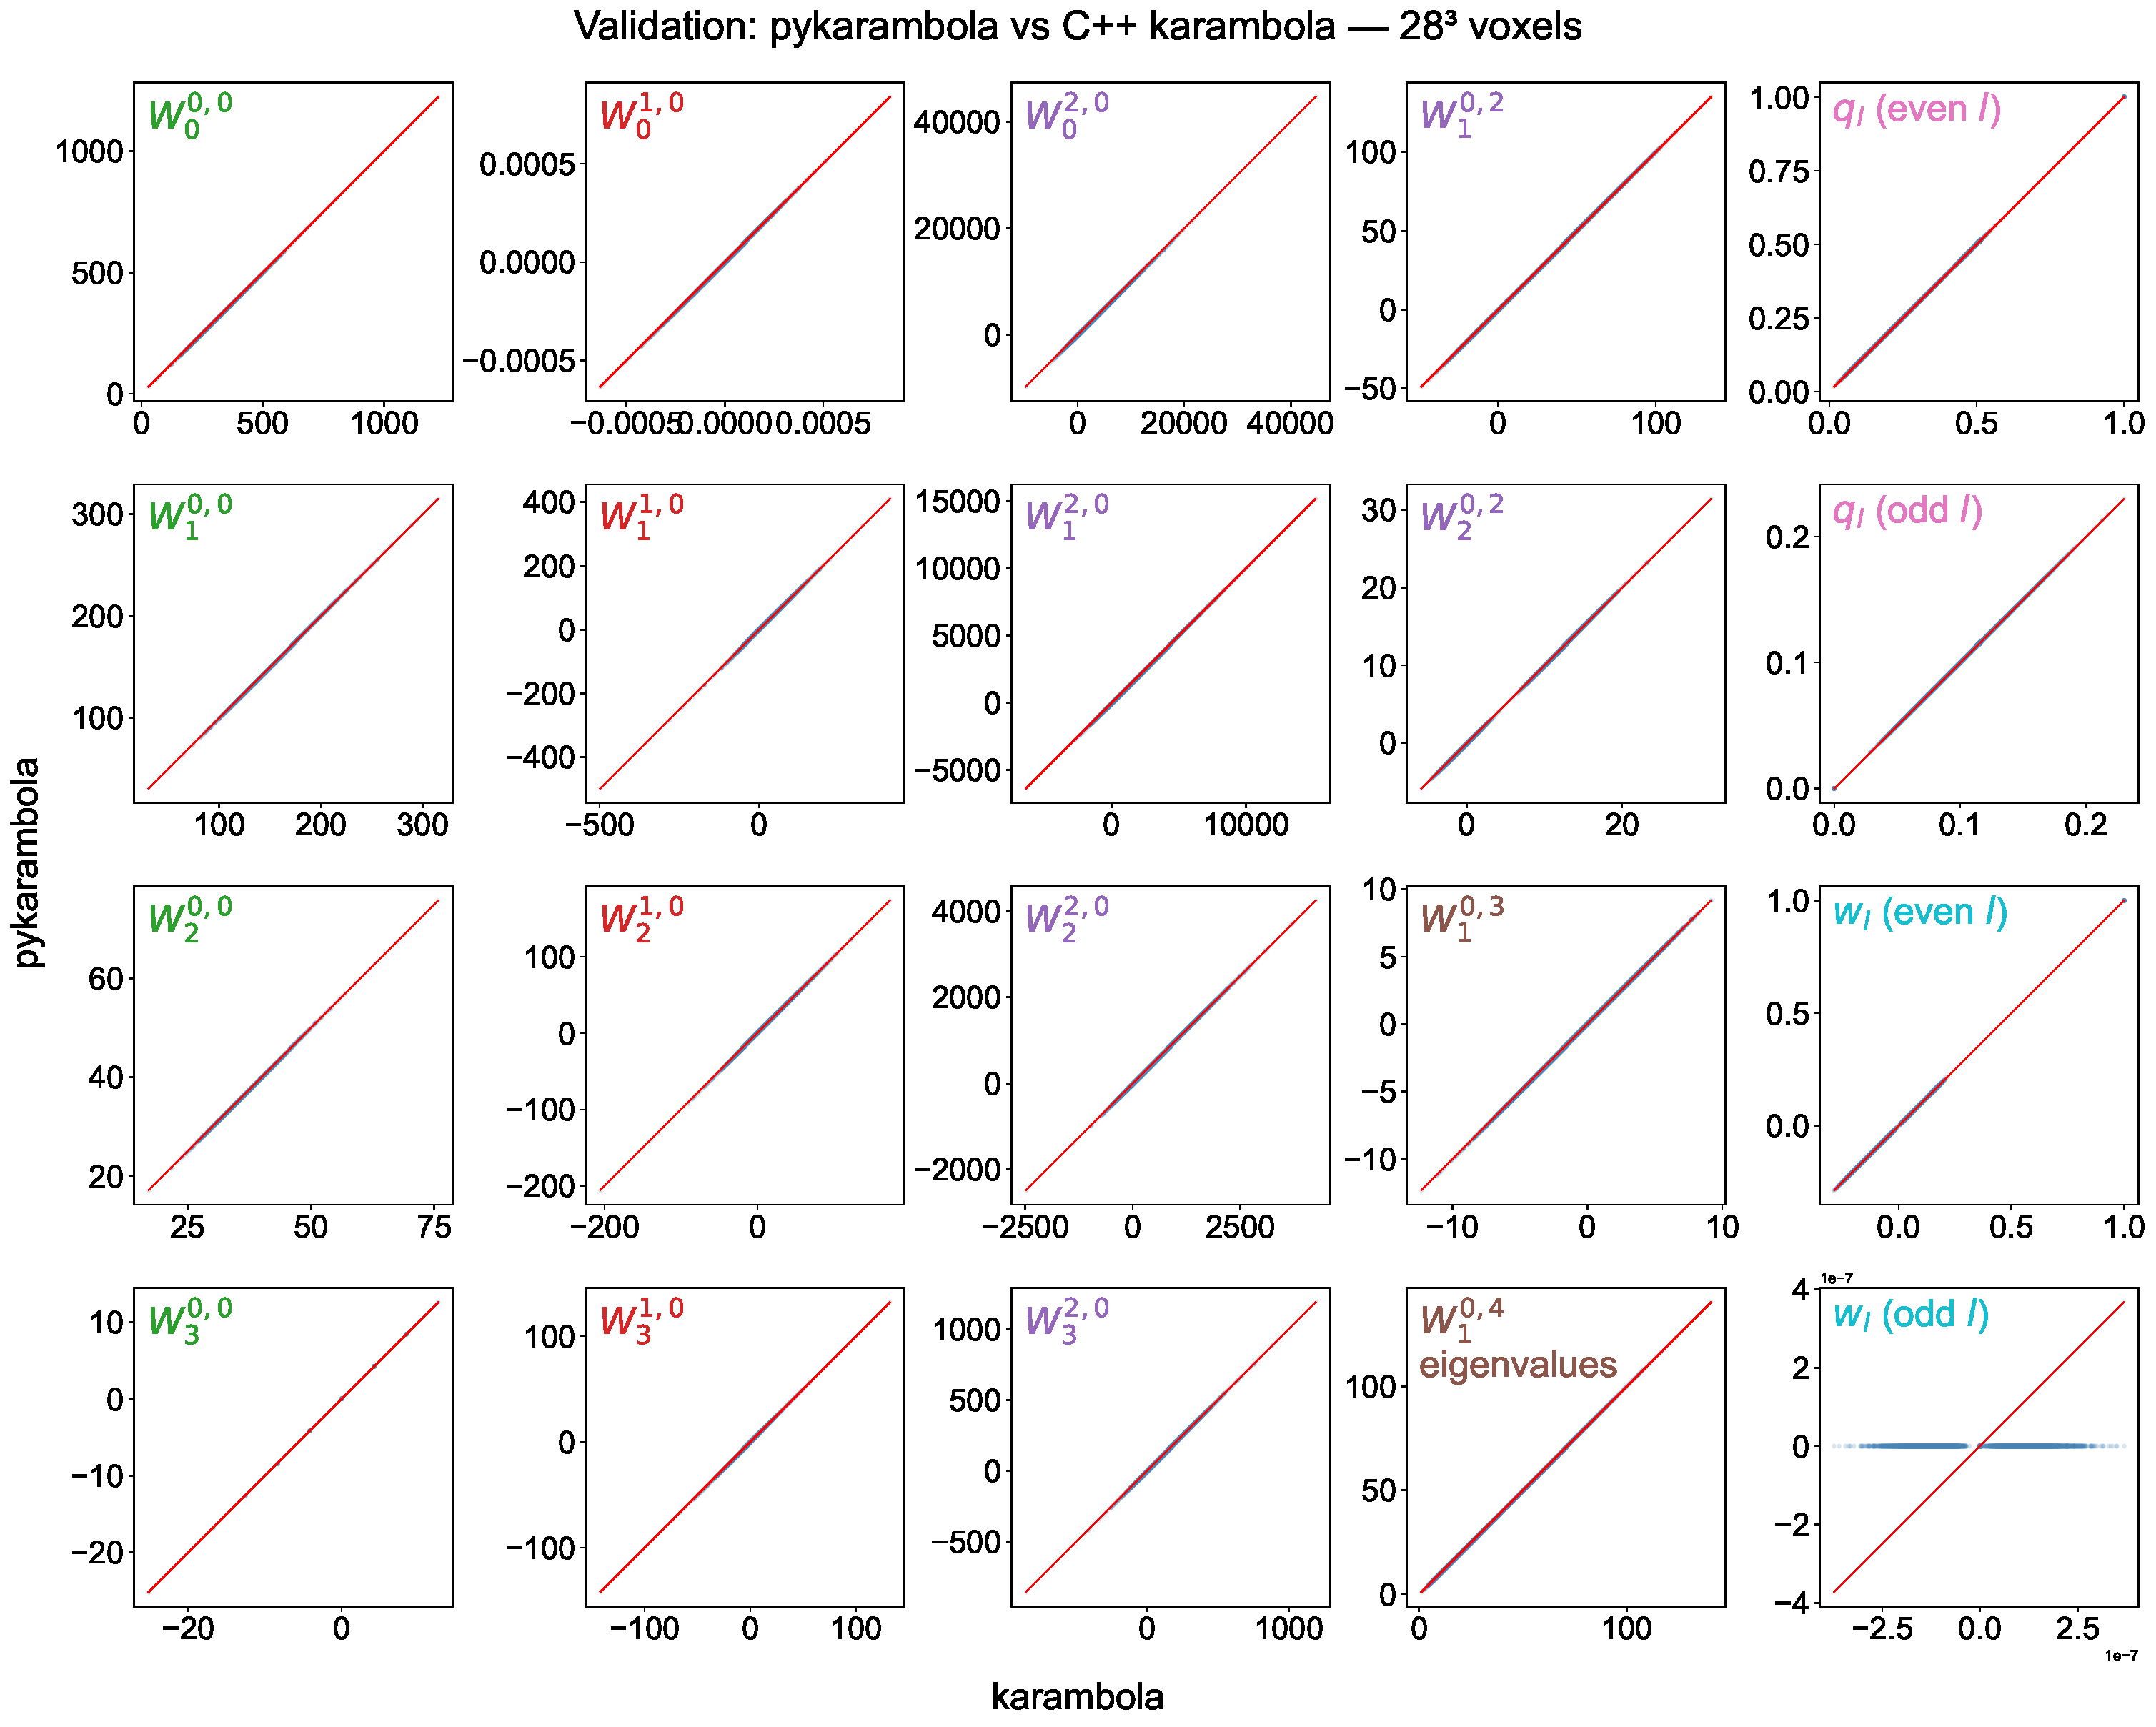
\includegraphics[width=0.95\textwidth]{notebooks/results/scatter_accuracy_paper.pdf}
\caption{Numerical accuracy of \texttt{pykarambola} relative to C++ \texttt{karambola}.
Each panel shows a scatter plot of values from identical analyses run in C++
(\texttt{karambola}, $x$-axis) and Python (\texttt{pykarambola}, $y$-axis) on
the AdrenalMNIST3D dataset (1{,}584 meshes, $28^3$ voxel resolution).
Columns correspond to feature groups: scalars ($W_\nu^{0,0}$),
vectors ($W_\nu^{1,0}$), rank-2 tensors ($W_\nu^{2,0}$, $W_\nu^{0,2}$),
and higher-rank quantities ($W_1^{0,3}$, $W_1^{0,4}$ eigenvalues, and spherical
Minkowski summary quantities $q_l$ and $w_l$).
Panel labels are shown in the top-left corner of each panel, colored by feature group.
The red diagonal indicates perfect agreement; all points fall on this line.
Equivalent agreement is observed at $64^3$ resolution (Supplementary Figure~\ref{fig:accuracy_supp}).}
\label{fig:accuracy}
\end{figure*}

\subsection*{Label-image API walkthrough}
To demonstrate the label-image API, we applied \texttt{minkowski\_tensors\_from\_label\_image} to a publicly available 3D fluorescence segmentation of a human induced pluripotent stem cell (hiPSC) in early anaphase/telophase from the Allen Cell Collection~\cite{viana2023integrated}.
The segmentation provides a two-channel binary mask at isotropic voxel spacing of 0.108~$\mu$m: one channel for the DNA (nucleus) and one for the cell body.

Figure~\ref{fig:labelimage} illustrates how the choice of labelling scheme directly determines what the tensors measure, using the DNA channel as a concrete example.
In case~(i), the binary DNA mask is cast to an integer array (\texttt{dna\_mask.astype(int)}) and passed with the default \texttt{autolabel=False}; because all non-zero voxels share label value~1, the function returns one tensor set describing the aggregate geometry of all chromosomal material ($V = 110~\mu\text{m}^3$, $A = 435~\mu\text{m}^2$, $\chi = 2$, $\beta_0^{2,0} = 0.118$).
In case~(ii), \texttt{scipy.ndimage.label(dna\_mask)} first assigns a unique integer to each connected component; the resulting three-valued label image is passed with \texttt{autolabel=False} (default), and the function returns three independent tensor sets --- one per DNA object.
Equivalently, case~(ii) can be achieved in a single call by passing the binary mask with \texttt{autolabel=True}, which instructs the function to detect connected components on the mesh internally without any preprocessing; the per-object tensors are numerically identical.
The per-object results reveal structure that is invisible in case~(i): object~1 ($V = 56~\mu\text{m}^3$, $\beta_0^{2,0} = 0.194$) is approximately twice the volume of objects~2 and~3 ($V \approx 27~\mu\text{m}^3$ each), which are more elongated ($\beta_0^{2,0} \approx 0.144$--$0.151$), consistent with sister chromatids caught mid-separation.
The anisotropy of the DNA objects is substantially higher than that of the cell body ($\beta_0^{2,0} = 0.277$).

This example demonstrates a general principle: identical binary image data yields fundamentally different morphometric results depending on label assignment, and the correct choice depends on the biological question.
Whole-structure morphometry (case~i) is appropriate when the aggregate shape is the object of interest; per-object morphometry (case~ii) is required when individual instances must be resolved, as in cell counting, organelle tracking, or shape clustering.
Both modes are supported by a single function call; the full worked example including mesh visualisation and Minkowski tensor additivity is provided in the accompanying notebook (notebook~\#17, Supplementary Material).
The pipeline from label image to triangulated mesh and Minkowski tensors is summarised in Figure~\ref{fig:pipeline}; the pykarambola output is directly compatible with standard bioimage segmentation tools such as cellpose~\cite{Stringer2021cellpose} and StarDist~\cite{Schmidt2018stardist}, whose instance segmentation outputs are integer label images of precisely the form accepted by \texttt{minkowski\_tensors\_from\_label\_image}.

\begin{figure}
\centering
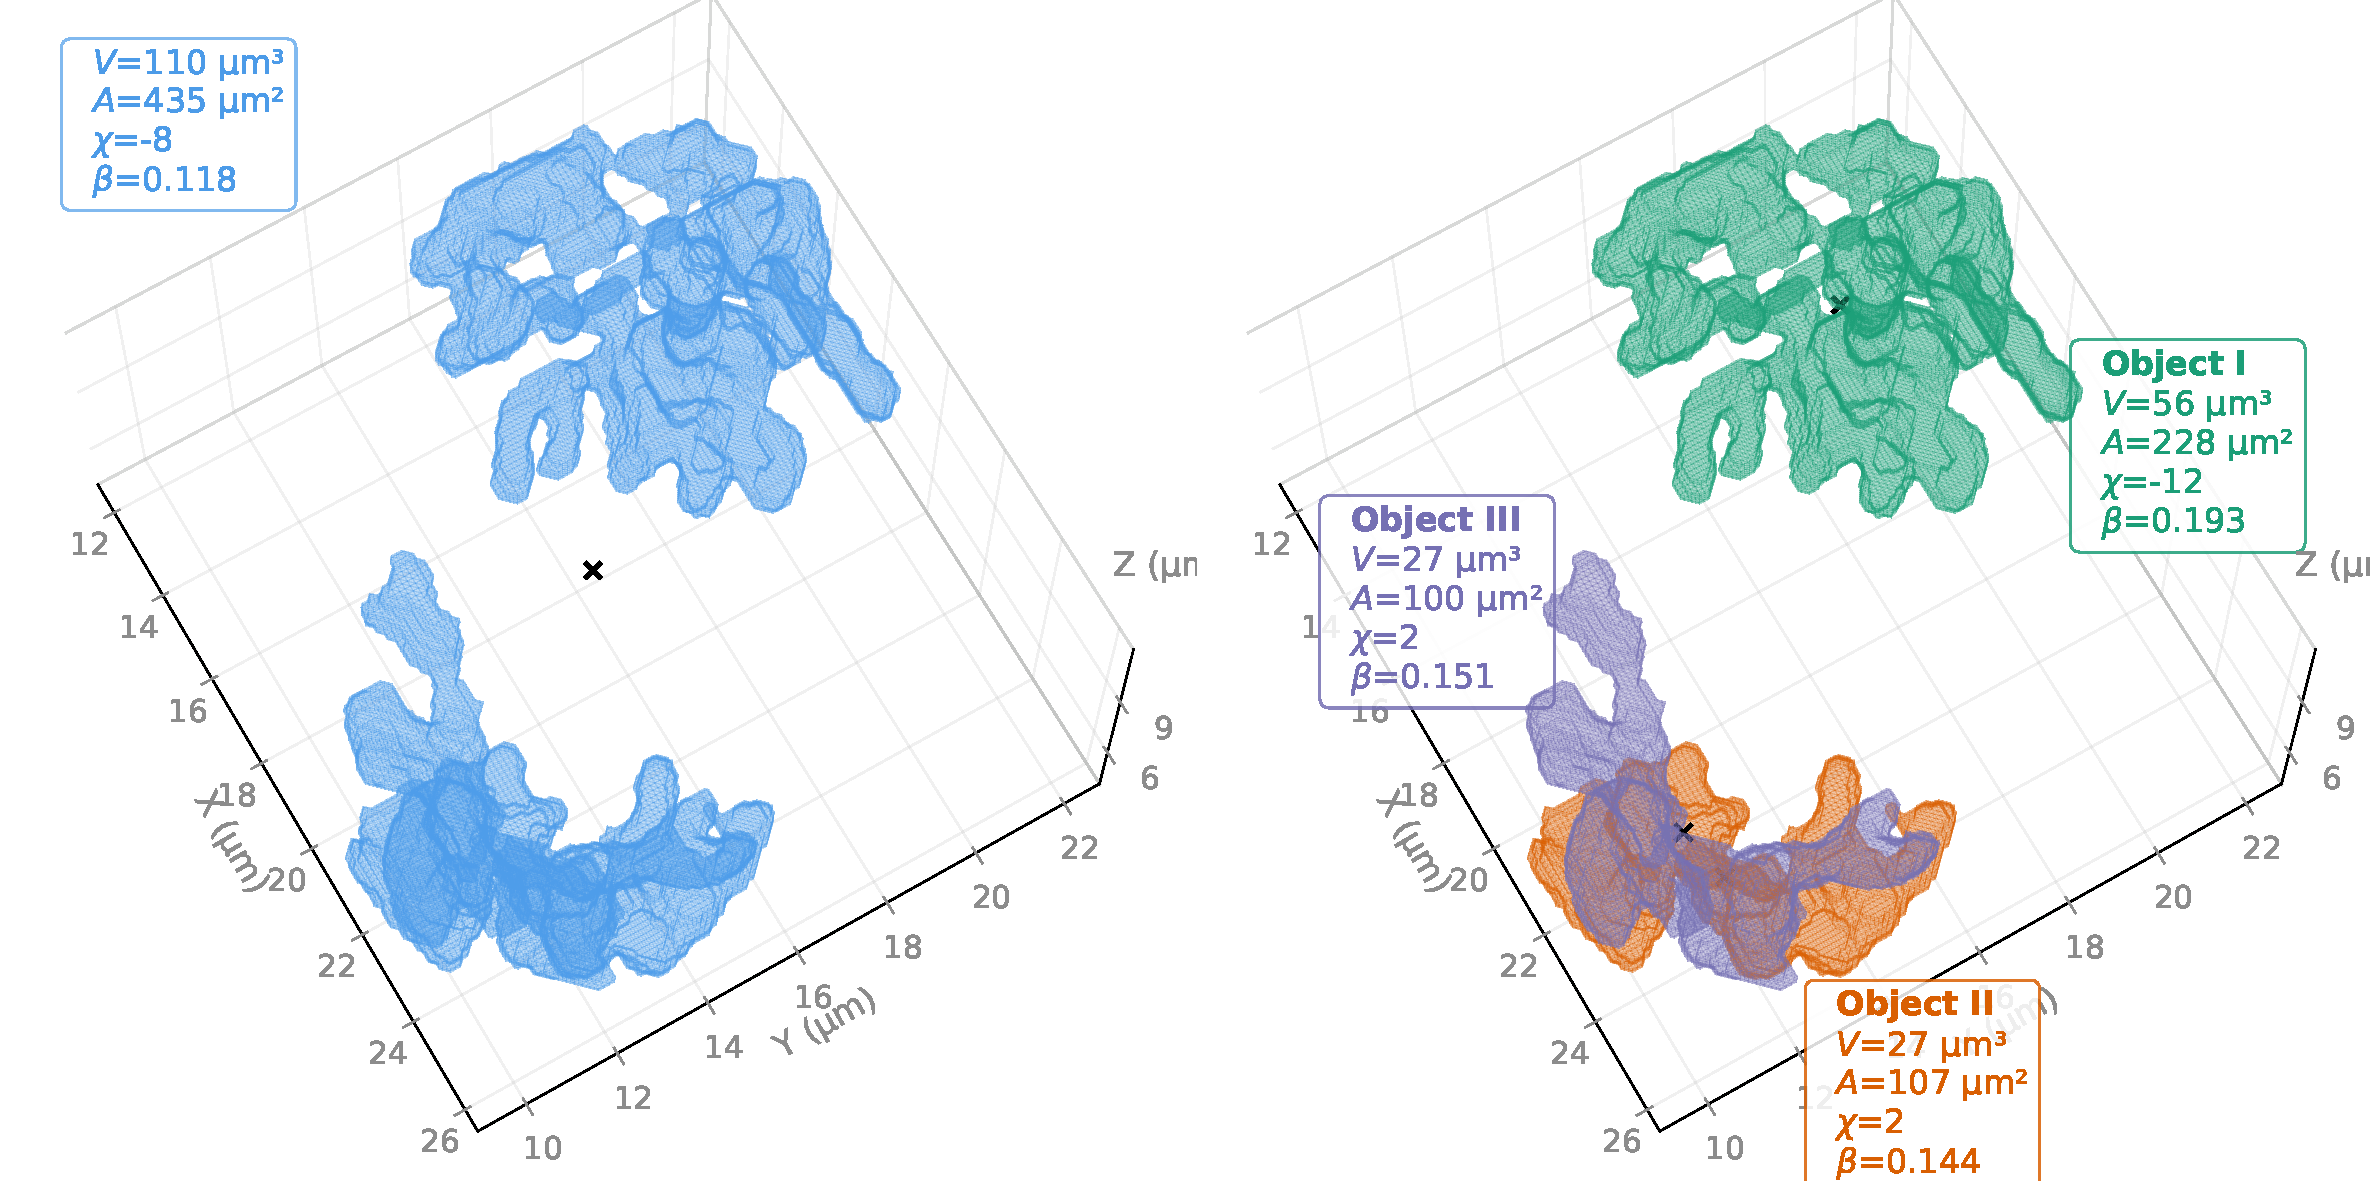
\includegraphics[width=\linewidth]{../assets/figure21.pdf}
\caption{%
  Label-image API applied to the DNA channel of a 3D fluorescence microscopy segmentation
  of a hiPSC in anaphase/telophase (Allen Cell Collection; isotropic voxel size 0.108\,\textmu m).
  (\textbf{a}) The entire DNA channel assigned as a single label;
  one set of Minkowski tensors describes the aggregate of all three DNA objects,
  with the volumetric centroid marked~($\times$).
  (\textbf{b}) Each DNA object assigned a distinct label via \texttt{scipy.ndimage.label};
  three independent tensor sets resolve per-object volume~($V$), surface area~($A$),
  Euler characteristic~($\chi$), and anisotropy index~($\beta$),
  with per-object centroids marked~($\times$).
  Objects~2 and~3 occupy different axial ranges (Z slices 40--72 and 78--110, respectively)
  and likely correspond to sister chromatids from the same chromosome.
}
\label{fig:labelimage}
\end{figure}


%% -------------------------------------------------------
\section*{Discussion}
%% -------------------------------------------------------
pykarambola makes Minkowski tensor morphometry directly accessible within the Python bioimage ecosystem by replacing a C++ binary with a pip-installable package that accepts NumPy arrays and returns plain Python dicts.
Beyond the interface change, the reimplementation extends input support to Wavefront OBJ, binary glTF, and STL files and adds a high-level label-image API that converts 3D segmentation outputs into per-object tensors in a single call.
The benchmark results show that on icospheres, the Cython-accelerated build was consistently faster than C++ karambola ($1.0$--$1.2\times$ speedup), while the pure-Python build was comparable or slightly slower at larger mesh sizes ($0.8$--$1.0\times$).
On the AdrenalMNIST3D dataset, pykarambola was faster than C++ karambola (2.8$\times$ at 28$^3$, 1.5$\times$ at 64$^3$), primarily because C++ karambola writes one result folder per object to disk.
The NumPy vectorization of the Minkowski tensor functionals over all triangles in a single array operation avoids per-triangle Python overhead and accounts for the compute-step parity with the C++ implementation.
The optional Cython extension targets only the graph-traversal steps of mesh initialisation, which resist vectorization; its benefit is therefore most pronounced for large meshes and batch analyses where initialisation cost dominates.
For interactive or small-scale use, the pure-Python build is sufficient and requires no compiled extension.

The primary limitation of pykarambola, inherited from karambola, is that it operates exclusively on triangulated surface meshes.
For label-image inputs, the surface is extracted by marching cubes, which introduces a discretization artefact: at typical fluorescence microscopy voxel sizes, the mesh is a piecewise-planar approximation of the true surface.
Tensor values therefore converge to their continuous limits as voxel resolution increases, and users working with low-resolution data should interpret results with this in mind.
Passing the physical voxel spacing via the \texttt{spacing} argument ensures that all length, area, and volume quantities are reported in physical units and are comparable across datasets acquired at different resolutions.

Future development directions include a napari plugin for interactive visualisation of tensor outputs alongside raw image data --- pykarambola's speed makes it well-suited for real-time feedback as users explore and annotate 3D segmentations, support for additional Minkowski tensor families beyond those available in karambola, and a streaming batch-processing mode for datasets too large to hold in memory simultaneously.
We invite the bioimage analysis community to adopt pykarambola as a drop-in morphometry step in existing segmentation pipelines and to contribute new measures, file format parsers, and downstream analysis notebooks via the project repository.


%% -------------------------------------------------------
\section*{Software availability}
%% -------------------------------------------------------
pykarambola is released under the GNU General Public License v3.0 or later (GPL-3.0-or-later) and is freely available at \url{https://github.com/Ishihara-SynthMorph/pykarambola}.
The package can be installed via the Python Package Index (PyPI) with \texttt{pip install pykarambola}.
Version 0.5.0, the version described in this paper, is permanently archived on Zenodo at \url{https://doi.org/10.5281/zenodo.20418801}.
Core dependencies are NumPy and SciPy; optional dependencies include Cython (for acceleration) and scikit-image (for label-image API).

%% -------------------------------------------------------
\section*{Data availability}
%% -------------------------------------------------------
All datasets used in this study are publicly available.
The AdrenalMNIST3D benchmark meshes are part of MedMNIST~\cite{Yang2023MedMNIST} and can be downloaded via the \texttt{medmnist} Python package.
The Allen Cell Collection segmentations are publicly available through the Allen Institute for Cell Science~\cite{viana2023integrated}.


\begin{acknowledgements}
pykarambola is a GPL\,3.0 derivative work of karambola, the C++ reference implementation by Schaller, Kapfer, and Schröder-Turk~\cite{Schaller2020karambola}.
This work was supported in part by an American Heart Association Career Development Award (grant 25CDA1432232) to K.I.

\textbf{AI tools disclosure.}
Claude Opus 4.5 and Claude Sonnet 4.6 (Anthropic) were used during this project for software and code development (Python port, refactoring, and test scaffolding) and for manuscript drafting and editing.
All AI-assisted outputs were reviewed, edited, and validated by the human authors before inclusion.
\end{acknowledgements}

\begin{contributions}
Y.K.\ and K.I.\ contributed equally to Software.
Y.K.: Methodology, Validation, Visualization, Writing -- original draft.
K.I.: Conceptualization, Funding acquisition, Project administration, Supervision, Writing -- review \& editing.
\end{contributions}

\section*{Bibliography}
\bibliography{references}

%TC:ignore
\onecolumn
\newpage

\section*{Word Counts}
\subsection*{Statistics on word count}
\detailtexcount

%TC:endignore
\newpage

\renewcommand{\thefigure}{S\arabic{figure}}
\setcounter{figure}{0}

\section{Supplementary Material}

\begin{figure*}
\centering
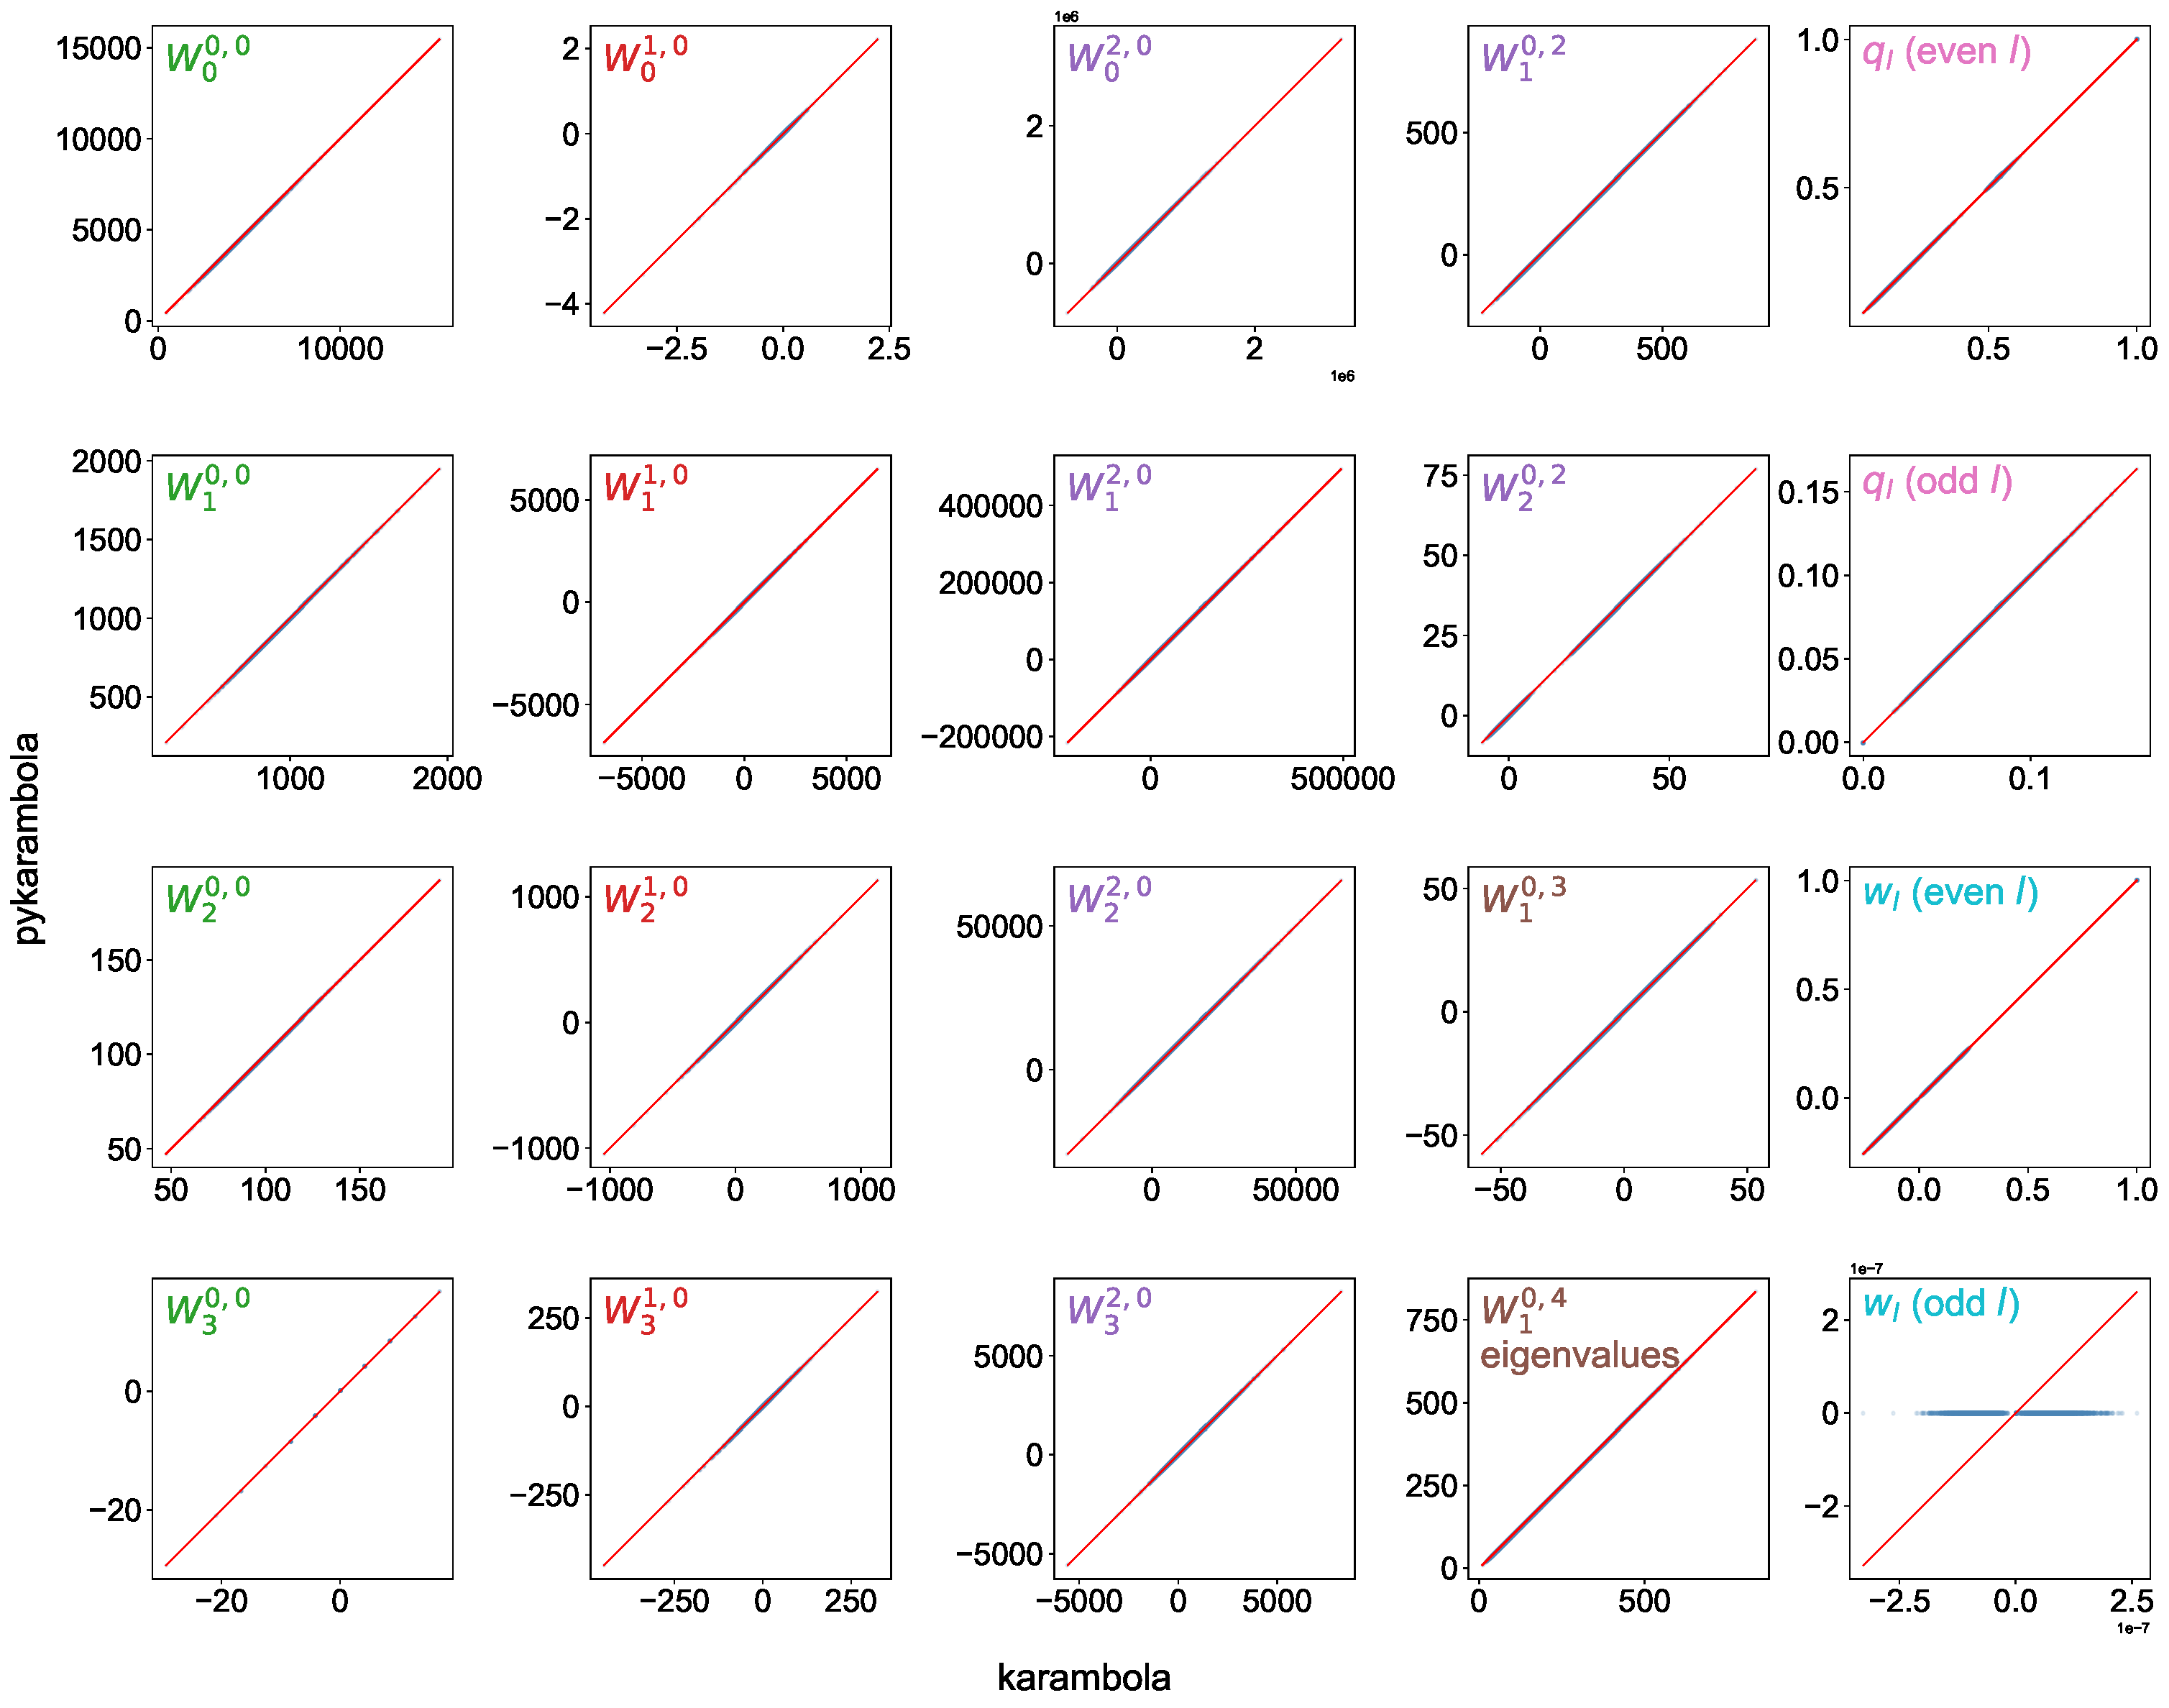
\includegraphics[width=0.95\textwidth]{notebooks/results/scatter_accuracy_paper_supplementary.pdf}
\caption{Numerical accuracy of \texttt{pykarambola} relative to C++ \texttt{karambola} at $64^3$ voxel resolution.
All panels and groupings are identical to Figure~\ref{fig:accuracy}.}
\label{fig:accuracy_supp}
\end{figure*}

\end{document}
